\documentclass[letter,11pt]{article}

\usepackage[spanish,es-nodecimaldot]{babel}
\usepackage[utf8]{inputenc}

\usepackage{lmodern}
\usepackage[T1]{fontenc}
\usepackage{textcomp}

\usepackage{framed}
\usepackage[svgnames]{xcolor}
\colorlet{shadecolor}{Gainsboro!50}

\usepackage{graphicx}
\usepackage{pstricks}

\usepackage{anysize}
\marginsize{3cm}{2cm}{2cm}{3cm}

\usepackage{siunitx}
\usepackage{amsmath}
\usepackage{array}

\usepackage{fancyhdr}
\usepackage{lastpage}
\pagestyle{fancy}
\fancyhf{}
\fancyhead[LE,RO]{Física Básica III}
\fancyfoot[CO,CE]{\thepage\ de \pageref{LastPage}}

\special{papersize=215.9mm,279.4mm}

\usepackage[
    pdfauthor={Carlos Eduardo Caballero Burgoa},%
    pdftitle={Física Básica III},%
    pdfsubject={Examen Final},%
    colorlinks,%
    citecolor=black,%
    filecolor=black,%
    linkcolor=black,%
    urlcolor=black,
    breaklinks]{hyperref}
\usepackage{breakurl}

\newcommand{\blankpage}{
\newpage
\thispagestyle{empty}
\mbox{}
\newpage
}

\renewcommand{\arraystretch}{1.2}

\begin{document}

\begin{center}
    {\Large \bf{Examen final}}
\end{center}

\noindent\fbox{%
    \parbox{\textwidth}{%
        Estudiante: CABALLERO BURGOA, Carlos Eduardo \\
        Carrera: Ingeniería Electromecánica \\
        Correo: cijkb.j@gmail.com
    }%
}

\vspace{0.5cm}

\begin{enumerate}
\item Dos pequeñas esferas de masa $m = 10 [g]$ están suspendidas de un punto
común mediante cuerdas de longitud $L = 50 [cm]$. Cuando cada una de las esferas
contiene la carga $q$, cada cuerda forma un ángulo $\theta = 10^\circ$ con la
vertical. Calcular la carga $q$.

\begin{figure}[!h]
\centering
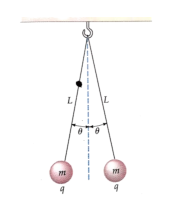
\includegraphics[scale=2.20]{resources/q1.eps}
\end{figure}

\begin{itemize}
    \item \textcolor{red}{$0.24 [\mu C]$.}
    \item $0.29 [\mu C]$.
    \item $0.32 [\mu C]$.
    \item $0.38 [\mu C]$.
\end{itemize}

\textbf{Solución:}

\begin{figure}[!h]
\centering
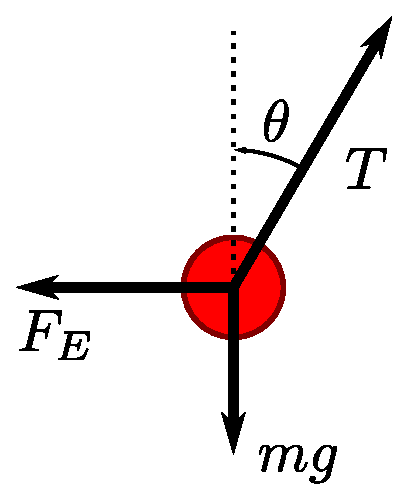
\includegraphics[scale=0.36]{resources/a1.eps}
\end{figure}

A partir del diagrama de cuerpo libre, sabemos:

\begin{equation*}
    \begin{cases}
        T\,cos(\theta)-mg = 0 \\
        T\,sen(\theta)-F_E = 0
    \end{cases}
\end{equation*}

Igualando ambas ecuaciones:

\begin{equation*}
    tan(\theta) = \frac{F_E}{mg}
\end{equation*}

Por la ley de \emph{Coulomb} sabemos:

\begin{equation*}
    F_E = \frac{1}{4\pi\epsilon_0}\frac{q^2}{r^2}
\end{equation*}

Ademas por propiedades trigonometricas sabemos:

\begin{equation*}
    sen(\theta) = \frac{r/2}{L}
\end{equation*}
\begin{equation*}
    r = 2L\,sen(\theta)
\end{equation*}

Juntando todas la ecuaciones:

\begin{equation*}
    mg\,tan(\theta) = F_E
\end{equation*}
\begin{equation*}
    mg\,tan(\theta) = \frac{1}{4\pi\epsilon_0}\frac{q^2}{r^2}
\end{equation*}
\begin{equation*}
    q^2 = 4\pi\epsilon_0 r^2 mg\,tan(\theta)
\end{equation*}
\begin{equation*}
    q = 2r\,\sqrt{\pi\epsilon_0\,mg\,tan(\theta)}
\end{equation*}
\begin{equation*}
    q = 2(2L sen(\theta)\,\sqrt{\pi\epsilon_0\,mg\,tan(\theta)}
\end{equation*}
\begin{equation*}
    q = 4L\,sen(\theta)\,\sqrt{\pi\epsilon_0\,mg\,tan(\theta)}
\end{equation*}
\begin{equation*}
    q = 4(0.5)\,sen(10^\circ)\,\sqrt{\pi\epsilon_0\,(0.01)(9.81)\,tan(10^\circ)}
      = \num{2.4086e-7} [C]
\end{equation*}

\item Un cuadripolo consta de dos dipolos próximos entre sí. La carga efectiva
en el origen es $-2q$ y las otras cargas sobre el eje ``y'' en $y = a$ e
$y = -a$ tienen valores de $q$. Tomando los valores $q = 1 [\mu C]$ y
$a = 1 [cm]$, hallar el valor del campo eléctrico en un punto sobre el eje $x$ a
gran distancia de manera que $x \gg a$.

\begin{figure}[!h]
\centering
\includegraphics[scale=2.20]{resources/q2.eps}
\end{figure}

\begin{itemize}
    \item $ 2.7/x$.
    \item $-2.7/x^2$.
    \item $ 2.7/x^3$.
    \item \textcolor{red}{$-2.7/x^4$.}
\end{itemize}

\textbf{Solución:}

Por la superposición de los campos electricos, tenemos:

\begin{equation*}
    E_T = \frac{1}{4\pi\epsilon_0}\left(\frac{q}{r^2}\right)\frac{x}{r}
        - \frac{1}{4\pi\epsilon_0}\left(\frac{2q}{x^2}\right)
        + \frac{1}{4\pi\epsilon_0}\left(\frac{q}{r^2}\right)\frac{x}{r}
\end{equation*}
\begin{equation*}
    E_T = \frac{1}{4\pi\epsilon_0}\left(\frac{2qx}{r^3}\right)
        - \frac{1}{4\pi\epsilon_0}\left(\frac{2q}{x^2}\right)
        = \frac{2q}{4\pi\epsilon_0}\left(
          \frac{x}{(a^2+x^2)^{3/2}}-\frac{1}{x^2}\right)
\end{equation*}
\begin{equation*}
    E_T = \frac{q}{2\pi\epsilon_0}\left(
          \frac{x}{[(x^2)(\frac{a^2}{x^2}+1)]^{3/2}}-\frac{1}{x^2}\right)
        = \frac{q}{2\pi\epsilon_0}\left(
          \frac{x}{x^3(\frac{a^2}{x^2}+1)^{3/2}}-\frac{1}{x^2}\right)
\end{equation*}
\begin{equation*}
    E_T = \frac{q}{2\pi\epsilon_0}\left[
          \frac{1}{x^2\left(\frac{a^2}{x^2}+1\right)^{3/2}}-\frac{1}{x^2}\right]
        = \frac{q}{2\pi\epsilon_0 x^2}\left[
          \left(\frac{a^2}{x^2}+1\right)^{-3/2}-1\right]
\end{equation*}

Haciendo una aproximación por expansión binomial:

\begin{equation*}
    (1 + x)^n \approx 1 + nx
\end{equation*}

Por tanto:

\begin{equation*}
    E_T = \frac{q}{2\pi\epsilon_0 x^2}\left[
          \left(1+\left(-\frac{3}{2}\right)\frac{a^2}{x^2}\right)-1\right]
        = \frac{q}{2\pi\epsilon_0 x^2}\left(-\frac{3a^2}{2x^2}\right)
\end{equation*}
\begin{equation*}
    E_T = -\frac{3qa^2}{4\pi\epsilon_0 x^4}
        = -\frac{3(1\mu)(0.01)^2}{4\pi\epsilon_0 x^4}
        = -\frac{2.6964}{x^4}
\end{equation*}

\item Una esfera uniformemente cargada de radio $R = 20 [cm]$ está centrada en
el origen con una carga $Q = 2 [mC]$. Determinar la fuerza resultante que actúa
sobre una línea uniformemente cargada, orientada radialmente y con una carga
total $q = 3 [\mu C]$ con sus extremos en $x = R$ y $x = R + d$, donde
$d = 10 [cm]$.

\begin{itemize}
    \item $1350 [N]$.
    \item \textcolor{red}{$ 900 [N]$.}
    \item $ 864 [N]$.
    \item $ 600 [N]$.
\end{itemize}

\textbf{Solución:}

\begin{figure}[!h]
\centering
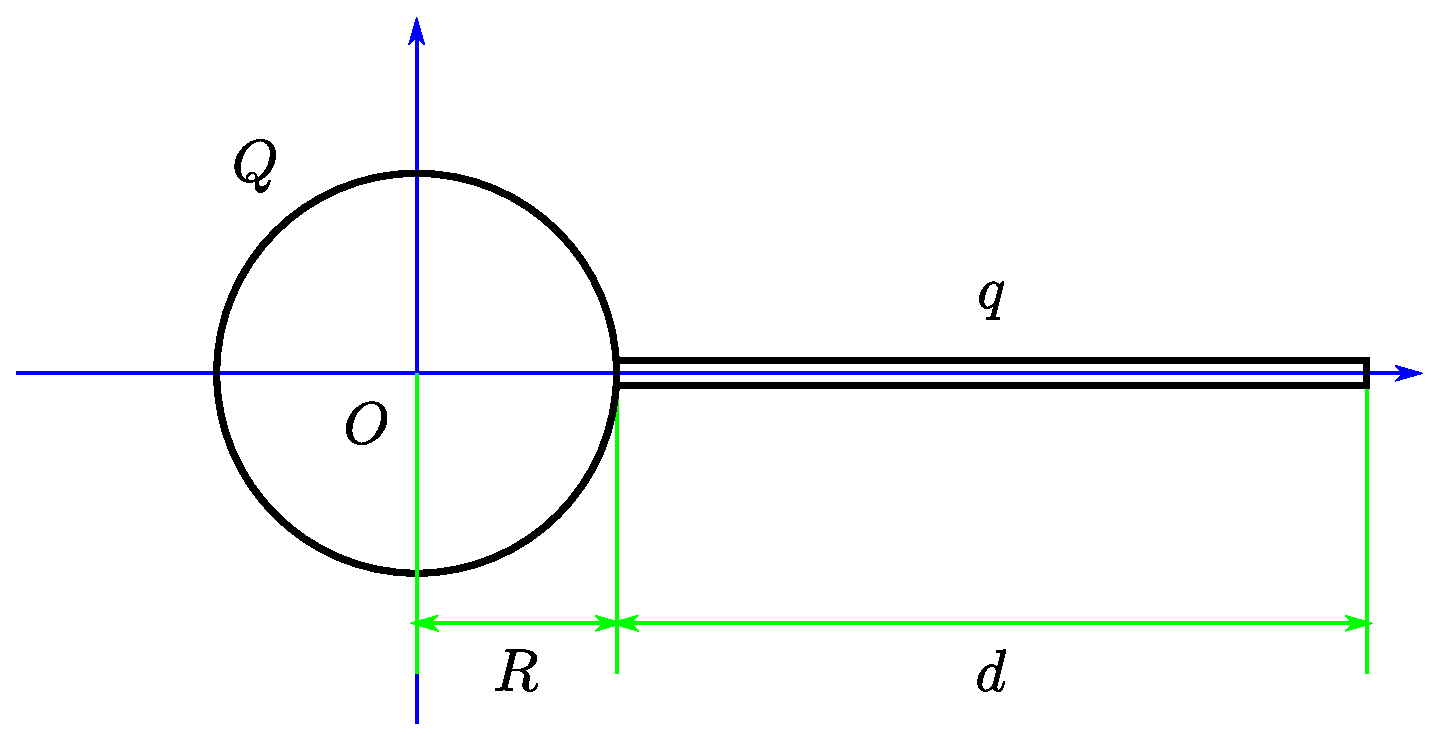
\includegraphics[scale=0.40]{resources/a3.eps}
\end{figure}

Sabiendo que la carga de una esfera con radio $R$ y carga $Q$ distribuida de
manera uniforme es:

\begin{equation*}
    E = \frac{1}{4\pi\epsilon_0}\frac{Q}{r^2};\,r > R
\end{equation*}

Calculando la fuerza ejercida:

\begin{equation*}
    dF = \frac{1}{4\pi\epsilon_0}\frac{Q}{r^2} dq
\end{equation*}

Considerando la densidad lineal:

\begin{equation*}
    \lambda = \frac{dq}{dr}
\end{equation*}
\begin{equation*}
    dq = \lambda dr
\end{equation*}

Por tanto:

\begin{equation*}
    dF = \frac{1}{4\pi\epsilon_0}\frac{Q}{r^2}\lambda dr
\end{equation*}
\begin{equation*}
    F = \int_{R}^{R+d} \frac{1}{4\pi\epsilon_0}\frac{Q}{r^2}\lambda dr
      = \frac{Q\lambda}{4\pi\epsilon_0} \int_{R}^{R+d} \frac{dr}{r^2}
      = \frac{Q\lambda}{4\pi\epsilon_0}\left(
        -\frac{1}{r}\Biggr|_{R}^{R+d}\right)
      = \frac{Q\lambda}{4\pi\epsilon_0}\left(-\frac{1}{R+d}+\frac{1}{R}\right)
\end{equation*}
\begin{equation*}
    F = \frac{Q\lambda}{4\pi\epsilon_0}\left(\frac{-R+R+d}{R(R+d)}\right)
      = \frac{Q\lambda}{4\pi\epsilon_0}\left(\frac{d}{R(R+d)}\right)
      = \frac{Q}{4\pi\epsilon_0}\left(\frac{q}{d}\right)
        \left(\frac{d}{R(R+d)}\right)
\end{equation*}
\begin{equation*}
    F = \frac{Qq}{4\pi\epsilon_0}\left(\frac{1}{R(R+d)}\right)
      = 898.7552 [N]
\end{equation*}

\item Una carga lineal semi-infinita de densidad uniforme
$\lambda = \num{1e-6} [C/m]$ está sobre el eje $x$ desde $x = 0$ hasta
$x = \infty$. Hallar la magnitud del campo eléctrico en el punto $x = 0 [m]$,
$y = 1 [m]$, en números enteros.

\begin{itemize}
    \item $12728 [N/C]$.
    \item $10523 [N/C]$.
    \item $ 8645 [N/C]$.
    \item $ 6019 [N/C]$.
\end{itemize}

\textbf{Solución:}

\item Cuatro cargas iguales $Q = 1 [\mu C]$ se encuentran en los vértices de un
cuadrado de lado $L = 10 [cm]$. Las cargas se dejan en libertad de una en una
siguiendo el sentido de las agujas del reloj alrededor del cuadrado. Se deja que
cada carga alcance su velocidad final a una gran distancia del cuadrado antes de
liberar la siguiente carga. Calcular la energía cinética final de la primera
carga liberada.

\begin{itemize}
    \item $487.28 [mJ]$.
    \item $243.64 [mJ]$.
    \item $153.64 [mJ]$.
    \item $ 90    [mJ]$.
\end{itemize}

\textbf{Solución:}

\item Una partícula de masa $m = \num{1e-9} [kg]$ y carga $Q = 1 [\mu C]$ está
localizada sobre el eje $x$ en $x = a$ ($a = 50 [cm]$), mientras que una segunda
partícula de igual masa y carga $-Q$ está localizada sobre el eje $x$ en
$x = -a$. Ambas se dejan en libertad en el tiempo $t = 0$. Calcular la magnitud
de la velocidad de la partícula cargada positivamente en $x = a/2$.

\begin{itemize}
    \item $6000 [m/s]$.
    \item $5000 [m/s]$.
    \item $4000 [m/s]$.
    \item $3000 [m/s]$.
\end{itemize}

\textbf{Solución:}

\item Dos condensadores idénticos de placas paralelas de $10 [\mu F]$ (cada uno)
reciben cargas iguales de $100 [\mu C]$ cada uno y luego se separan de la fuente
de carga. Mediante un cable se conectan sus placas positivas y mediante otro sus
placas negativas. Calcular la energía final almacenada en el sistema.

\begin{itemize}
    \item $1000    [\mu J]$.
    \item $ 832.64 [\mu J]$.
    \item $ 616.09 [\mu J]$.
    \item $ 476.19 [\mu J]$.
\end{itemize}

\textbf{Solución:}

\item Un condensador está formado por dos cilindros concéntricos de radios
$a = 2 [mm]$ y $b = 4 [mm]$, siendo su longitud $L = 10 [m]$. El cilindro
interior posee una carga $Q =1 [\mu C]$ y el cilindro exterior una carga $-Q$.
La región comprendida entre los cilindros está llena con un dieléctrico de
constante $k = 3$. Si el dieléctrico se desplaza (sin fricción), calcule la
energía que se necesita para extraer el dieléctrico.

\begin{itemize}
    \item $352,23 [\mu J]$.
    \item $394.37 [\mu J]$.
    \item $415.89 [\mu J]$.
    \item $448.62 [\mu J]$.
\end{itemize}

\textbf{Solución:}

\item El espacio comprendido entre dos cilindros metálicos metálicos coaxiales
de longitud $L = 50 [cm]$ y radios: $a = 1.5 [cm]$ y $b = 2.5 [cm]$ se llena
totalmente de un material de resistividad igual a $30 [\Omega m]$. Determinar la
intensidad de corriente entre los dos cilindros si se aplica una diferencia de
potencial de $10 [V]$ entre éstos.

\begin{itemize}
    \item $2.05 [A]$.
    \item $1.69 [A]$.
    \item $1.28 [A]$.
    \item $1.03 [A]$.
\end{itemize}

\textbf{Solución:}

\item Un disco no conductor de masa $M$ y radio $R = 10 [cm]$ tiene una densidad
de carga superficial uniforme de $6 [\mu C/m^2]$ y gira con una velocidad
angular de $360 [rpm]$ alrededor de su eje. Calcular el momento magnético de la
carga total del disco.

\begin{itemize}
    \item $45.24 [pA m^2]$.
    \item $41.08 [pA m^2]$.
    \item $38.45 [pA m^2]$.
    \item $33.33 [pA m^2]$.
\end{itemize}

\textbf{Solución:}

\end{enumerate}

\end{document}

